\documentclass[11pt,a4paper]{article}
\usepackage{graphicx}
\usepackage{xcolor}
\usepackage{geometry}
\usepackage{amsmath}
\usepackage{amssymb}
\usepackage{booktabs}
\usepackage{tabularx}
\usepackage{adjustbox}
\usepackage{enumitem}
\usepackage{microtype}
\usepackage[numbers,sort&compress]{natbib}
\usepackage[colorlinks=true,linkcolor=blue!60!black,citecolor=blue!60!black,urlcolor=blue!60!black,bookmarks=true,unicode=true]{hyperref}
\geometry{a4paper, top=2.5cm, bottom=2.5cm, left=2.5cm, right=2.5cm}
\widowpenalty=10000
\clubpenalty=10000

\newcommand{\som}{\textsc{Somnium}}
\newcommand{\resnorm}{\mathrm{res}_{\mathrm{norm}}}

\begin{document}

% ---------- title block ----------
\begin{center}
{\LARGE\bfseries Somnium: A Recurrent World Model\\[5pt] that Learns to Dream Before It Wakes}\\[13pt]
{\large Xiaoming (Will) Wang}\\[5pt]
{\small Independent Researcher}\\[2pt]
{\small \texttt{xwang755@asu.edu} $\cdot$ \url{https://github.com/wilberforce1900/somnium}}\\[5pt]
{\small October 2026}\\[3pt]
{\small v1.0 preprint $\cdot$ DOI: \href{https://doi.org/10.5281/zenodo.23278220}{10.5281/zenodo.23278220}}
\end{center}
\vspace{2pt}
\noindent\rule{\textwidth}{0.4pt}
\vspace{2pt}

\begin{abstract}
\noindent We train a small non-Transformer world model, \som{}, under a developmental curriculum: \emph{chaos $\rightarrow$ dream $\rightarrow$ wake}. A single recurrent substrate carries two dynamics---fast streaming expansion (\emph{yang}) and energy-relaxation contraction (\emph{yin})---softly mixed by a gate; prediction happens in latent space (JEPA-style next-latent), and training begins with a \emph{dream phase} of self-generated rollouts before any real environment interaction. Dream-first pretraining reliably cuts the real-interaction steps needed to reach a fixed accuracy by ${\sim}60\%$: replicated across five independent runs at 16K parameters (ratios 0.39--0.42 against a pre-registered threshold of 0.6). Three further lines of evidence---a scale ladder, a dose-scaling control, and 871-round autonomous growth runs---converge on the same conclusion: the advantage is \emph{capacity-bound}. It disappears at 210K--3.2M parameters, scaling the dream budget with width does not restore it, and a dream-grown model that widens from 64 to 486 dimensions stays healthy while the step to 1024 destabilizes training. Alongside the positive result we report a registry of pre-registered negative results: a 64-entry VQ situation codebook hurts training, a learned gate yields no accuracy gain over fixed dynamics (though its polarity is a load-bearing developmental marker we characterize as a ratchet), and feeding dream statistics back into sampling does not improve calibration. All hypotheses, thresholds, and outcomes---including two overnight infrastructure failures---are logged in a public run registry. A theory that can be killed is a theory that can evolve.
\end{abstract}

\vspace{2pt}
\noindent\textbf{Keywords:} world models; pretraining; self-supervised learning; continual learning; sleep-inspired computation; pre-registration; negative results

\section{Introduction}\label{sec:intro}

Should a model meet the world awake or asleep? Mammalian development suggests an ordering: spontaneous, self-generated activity (retinal waves, hippocampal replay) precedes and shapes later sensorimotor learning~\cite{blankenship2009,wilson1994}. Sleep research offers candidate mechanisms---synaptic homeostasis~\cite{tononi2014}, reverse learning~\cite{crick1983}, consolidation via replay~\cite{rasch2013}. In machine learning, world models trained by latent imagination~\cite{hafner2023} and self-supervised objectives in representation space~\cite{lecun2022,assran2023} echo pieces of this story, but the developmental question---\emph{does a model that dreams before it wakes learn more efficiently from its later waking data?}---is rarely asked directly.

We built \som{} to ask it under a discipline borrowed from clinical research: \textbf{pre-registered ablations with a public outcomes registry}. Every claim in this paper was registered with a threshold before the run that tested it; every negative result is retained and reported. The contributions are:

\begin{enumerate}[leftmargin=1.6em,itemsep=1pt,topsep=2pt]
\item \textbf{Architecture} (\S\ref{sec:arch}). A non-Transformer world model: one recurrent substrate with dual dynamics (streaming expansion / energy relaxation), gate-mixed; JEPA-style next-latent training with $O(1)$ state; a function-preserving width-growth operator; parameter count $3d_h^2 + O(d_h)$.
\item \textbf{A replicated, capacity-bound positive result} (\S\ref{sec:exp}). Dream-first pretraining reaches a wake-only model's final accuracy with ${\sim}40\%$ of the real interactions, replicated $5\times$ at 16K parameters across two compute platforms. A scale ladder (16K/210K/3.2M), a dose-scaling control ($4\times$/$16\times$ dream budget), and autonomous growth runs independently agree: the advantage is real but \emph{capacity-bound}, consistent with its mechanism being energy smoothing---an initialization effect that large models do not need.
\item \textbf{A registry of pre-registered negative results} (\S\ref{sec:neg}). VQ situation codebooks hurt training; learned gating gives no accuracy gain (but its polarity is an emergent developmental marker: a one-way ratchet from corrective to feed-forward regimes); dream-statistics feedback does not improve calibration.
\item \textbf{An autonomous overnight protocol} (\S\ref{sec:night}) in which the model trains itself through self-probes, expands its own width by dreaming, and---in the second night---detects its own numerical divergence and rolls back to its last healthy self.
\end{enumerate}

We emphasize what this paper is \emph{not}: \som{} is a 16K--3.2M-parameter model on procedural gridworlds. Nothing here claims general-purpose intelligence. The point is methodological: with pre-registration and honest registries, a two-day single-GPU project can produce claims that replicate, boundaries that are measured rather than assumed, and failures that accumulate into design knowledge.

\section{Architecture}\label{sec:arch}

\subsection{One substrate, two dynamics}

\som{} has no attention and no token sequence. Its core is a single latent state $h_t \in \mathbb{R}^{d_h}$ updated once per environment step by soft-mixing two dynamics that \emph{share all parameters} (a deliberate contrast with dual-network designs; cf.\ the finding that a single tiny recursive network outperforms a biologically-inspired hierarchy~\cite{jolicoeur2025}):

\begin{align}
h_{t+1} &= h_t + \alpha_t\,\Delta^{\text{yang}}_t + (1-\alpha_t)\,\Delta^{\text{yin}}_t \label{eq:mix}\\
\Delta^{\text{yang}}_t &= \mathrm{dt}\cdot\tanh\!\big(W_c [h_t; e(o_t); a_t]\big) \label{eq:yang}\\
\Delta^{\text{yin}}_t &= -\mathrm{lr}\cdot\nabla_{h} E(h)\big|_{h=h_t}, \qquad \alpha_t = \sigma\!\big(g([h_t; x_t])\big) \label{eq:yin}
\end{align}

\noindent where $e(\cdot)$ is an encoder shared with the training target, $W_c$ a linear cell, $E$ a small MLP energy head, and $g$ a linear gate initialized at $\sigma(0)=0.5$ (born half-and-half). Equation~\eqref{eq:mix} is the model's entire per-step computation: the recurrent state is $O(1)$, ``thinking longer'' costs compute but never parameters, and the parameter count is $3d_h^2 + 52d_h + 296$ for our 8-dimensional observations and 4 actions---e.g.\ 16K at $d_h{=}64$, 3.2M at $d_h{=}1024$.

\subsection{Training objective}

Training is JEPA-style prediction in latent space, never next-token and never pixel reconstruction:
\begin{equation}
\mathcal{L} = \big\|h_{t+1} - \mathrm{sg}\big(e(o_{t+1})\big)\big\|^2
+ \lambda_r \big(\hat r_{t+1} - r_{t+1}\big)^2
+ \lambda_v \, \mathcal{N}\!\big(\hat r_{t+1}, \hat\sigma^2_{t+1};\, r_{t+1}\big)
+ \lambda_d \big(\hat o_{t+1} - o_{t+1}\big)^2 ,
\label{eq:loss}
\end{equation}
with $\mathrm{sg}(\cdot)$ a stop-gradient on the target (v0; no EMA teacher yet), $\hat\sigma$ a heteroscedastic uncertainty head used only for probes and abstention experiments, and $\hat o$ a low-weight observation decode used only to close the loop for planning probes. Each training sequence begins from a noise sample (the ``chaos'' stage): $h_0 \sim \mathcal{N}(0, I)$.

\subsection{The dream phase}\label{sec:dreamphase}

Before the first real interaction (\emph{dream-first}) the model runs self-generated rollouts with four independently togglable components: \textbf{imagination} (latent rollouts from the noise prior; the effective term turns out to be energy smoothing, \S\ref{sec:disc}), \textbf{consolidation} (replay distillation from the episode buffer), \textbf{reverse learning} (noise-augmented replay, after~\cite{crick1983,shin2017}), and \textbf{rehearsal} (oversampling rare transitions). Three schedules are compared throughout: \emph{wake-only}, \emph{dream-first} (dream pretraining, then wake-only), and \emph{alternate} (a dream phase after each wake cycle). A fairness note applies to all comparisons: dream schedules receive extra offline gradient steps; the metric is always \emph{real environment interactions}.

\subsection{Function-preserving growth}

To let the model widen itself, we use a Net2Net-style operator~\cite{wei2016}: new latent dimensions copy a random source dimension in all \emph{producer} weights (encoder output, cell output) while all \emph{consumer} weights receive zero columns. At zero noise the update map is bit-exact before and after growth (verified in tests); with small noise on new rows only, perturbation is $O(\varepsilon)$ and new dimensions wake up through gradients. Growth multiplies the dream budget by 1.5 (``the dream deepens as the dreamer grows''); the optimizer is rebuilt at each growth event.

\section{Experiments}\label{sec:exp}

\subsection{Protocol}

Environments are procedural gridworlds (5--12 cells; 8-dim observations: position, goal and hazard offsets, clock; slippery actions; rare hazard teleports) and DFS mazes. All comparisons hold the wake data stream identical across schedules. The primary metric is the \emph{steps-to-target ratio}: real interaction steps for a schedule to first reach the wake-only model's final accuracy, divided by the wake-only total. Thresholds were committed before each run: ratio $\le 0.6$ (i.e., a ${\ge}40\%$ saving) counts as positive. Code, registry, and per-run records: \url{https://github.com/wilberforce1900/somnium}.

\begin{figure}[t]
\centering
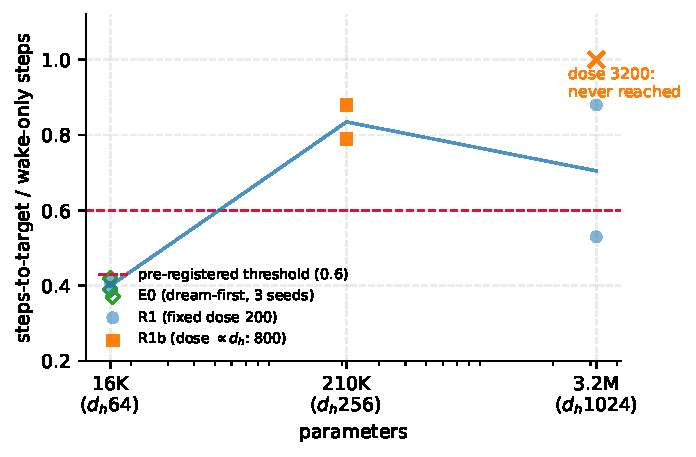
\includegraphics[width=0.62\textwidth]{figs/fig_scale.pdf}
\caption{\textbf{Dream advantage is capacity-bound.} Steps-to-target ratio (lower is better; pre-registered threshold 0.6 dashed). At 16K parameters dream-first reaches wake-only's final accuracy with ${\sim}40\%$ of the interactions (five independent runs across two platforms). At 210K/3.2M the advantage fades; scaling the dream budget with width (R1b) does not restore it, and at the largest scale the highest dose never reaches the target.}
\label{fig:scale}
\end{figure}

\subsection{Dream-first cuts real interactions by 60\% (at 16K)}

In the base configuration ($d_h{=}64$, ${\sim}5.3$K real steps total), dream-first reaches wake-only's final latent MSE using 39\%, 39\%, and 42\% of the real interactions (three seeds; final MSE 0.235 vs.\ 0.905 at equal steps). A cross-platform replication on an L4 GPU reproduced 0.41/0.39 with the identical configuration---a bit-exact determinism check. The \emph{alternate} schedule shows the same direction (0.77) without passing threshold: the benefit concentrates in \emph{pre-training}, not in interleaving. Component decomposition (six variants, pre-registered) attributes the sequential-learning benefit to replay components (consolidation $+6.1$pp, reverse learning $+6.0$pp, rehearsal $+5.3$pp on old-task improvement) while imagination contributes nothing there---its contribution is confined to the birth-time sample efficiency above, a division of labor we summarize as \emph{imagination is for being born; replay is for keeping what waking taught}.

\subsection{The advantage is capacity-bound}\label{sec:scale}

Figure~\ref{fig:scale} shows the scale ladder ($d_h \in \{64, 256, 1024\}$, two seeds each): ratios 0.41/0.39, 0.88/0.79, 0.88/0.53. Two confounds were closed by pre-registered controls:

\textbf{Dose.} Because the dream budget was fixed at 200 phases while width grew, we re-ran with dose $\propto d_h$ (200/800/3200). Outcome: unchanged at 210K (0.88/0.79, bit-identical trajectories' summary values), and at 3.2M the $16\times$ dose \emph{never reaches} the target (slightly worse than fixed dose). Under-dosing is not the explanation.

\textbf{Task saturation.} Wake-only final accuracy is flat in width (MSE 0.89/0.98/1.00): the environment family saturates near a few hundred dimensions, compressing any sample-efficiency advantage.

\subsection{Dream-grown models hit the same wall}\label{sec:night}

In autonomous overnight runs the model chose its own environment difficulty from four self-probes (normalized residual $\resnorm = \|h - e(o')\|/\sqrt{d_h}$, uncertainty $\hat\sigma$, coverage, gate polarity $\alpha$) and grew its width after two consecutive improving rounds. Night~1 (871 rounds, no safeguards) grew healthily from 64 to 486 ($\resnorm$ band 0.29--0.60), then the step to 1024 exploded the residual $6.8\times$; 667 subsequent rounds of self-repair halved it without recovery, with the gate pinned at the corrective pole ($\alpha \approx 0$) throughout. Night~2 (guard rails: growth only when $\resnorm < 0.6$, an anti-starvation rule for environment choice, gradient clipping, and rollback-to-last-healthy-self on divergence) grew to 729 while healthy, explored the environment grid to its ceiling, and---after an unclipped divergence late in the night---\emph{detected the failure via its own $\hat\sigma \to \infty$ probe and restored itself from its round-800 checkpoint}. Figure~\ref{fig:night} shows both trajectories.

\begin{figure}[t]
\centering
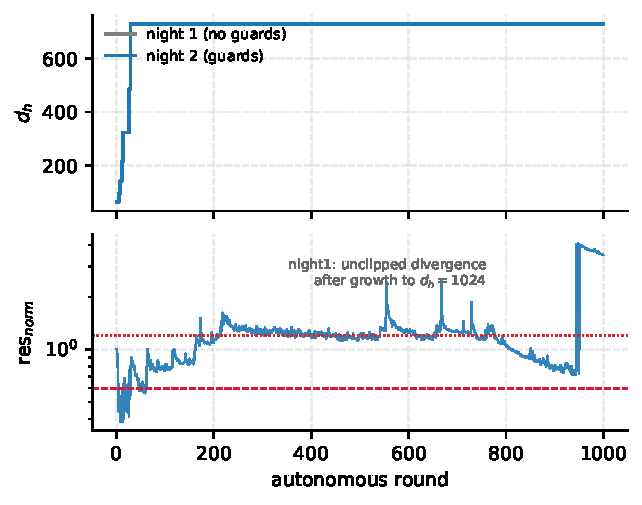
\includegraphics[width=0.62\textwidth]{figs/fig_overnight.pdf}
\caption{\textbf{Two nights of autonomous self-training.} Top: width $d_h$ over rounds (growth events). Bottom: normalized residual (log scale). Night 1: healthy growth to 486, destabilization at 1024, 667 rounds of unrecovered self-repair. Night 2 (guards + clipping + rollback): growth to 729 while healthy; the divergence near round 870 is rolled back to the last healthy self (round 800) and training continues below the band.}
\label{fig:night}
\end{figure}

\section{Negative results registry}\label{sec:neg}

All thresholds were pre-registered; all results retained.

\textbf{A1 --- 64-entry VQ situation codebook (``hexagram'' discrete planning layer).} Motivated by treating situations as a discrete transition graph over which a slow planner searches (value iteration over 64 codes, Xiantian binary encoding). Outcome at two seeds: the \emph{baseline without a codebook} reaches 0.406 success on long-horizon navigation while every codebook configuration scores $\le 0.094$; ablations show the VQ commitment loss \emph{damages the continuous model during training}. Two planner implementations (direct code scoring; potential-shaped search~\cite{ng1999}) failed a pre-launch check against an equal-compute control. Demoted to a read-only interpretability layer.

\textbf{A2 --- learned dual-mode gating.} Learned gate vs.\ fixed single-mode at equal parameters: $+0.9$pp / $-0.8$pp on two tasks against a $+2$pp threshold. The gate \emph{learns} (it settles at $\alpha \approx 0.3$) but converts to no accuracy. The interesting residue is what the gate encodes: polarity is \emph{co-adapted} (forcing a wake-trained model to the yang pole at inference inflates prediction error $4.4\times$), and it behaves as a \textbf{one-way developmental ratchet}---both schedules slide to the corrective (yin) pole early in training ($\alpha \to 0.17$); dream-pretrained models then ratchet to the feed-forward pole ($\alpha \to 0.96$) while wake-only models stay corrective; injecting a new task does \emph{not} reopen the gate. The gate is a stage marker, not an online ``do-I-know-this'' meter: a falsification we ran before believing it.

\textbf{A5 --- reading dreams to guide sampling.} Feeding dream-log statistics back (coverage-blind-spot bias of imagination; inverse-coverage-weighted replay) against matched controls: first implementation was mechanically inert (the imagination objective is content-insensitive); the second verifiably changed sampling but produced \emph{zero} calibration gain. Root cause: the uncertainty head is calibrated out of the box (95\% interval coverage 95--97\%), leaving no headroom to improve; per-window error discrimination was unstable across seeds ($-0.12$ vs.\ $+0.72$). Demoted to an observation layer.

\section{Discussion}\label{sec:disc}

\textbf{Mechanism.} Ablations localize the dream-first benefit to the energy-smoothing term of imagination (the anti-collapse variance floor was provably never active): pretraining flattens the energy landscape that the yin dynamics descend, i.e., it shapes the geometry the wake phase will optimize in. This is an initialization effect, which is exactly why it is capacity-bound---large models buy the same geometry with data. The alignment with sleep theory is comfortable but we state it flatly: what we implement is energy smoothing plus replay~\cite{tononi2014,crick1983,shin2017}; no claim about consciousness is made or implied, and we regard ``AGI as the awakening of silicon life'' as poetry, not prediction.

\textbf{Boundaries.} Toy environments; two seeds at scale; no external architecture baseline (the natural next control is a parameter-matched small transformer); compute asymmetry between dream and wake schedules is documented rather than eliminated; the registry contains two infrastructure failures (a shell incompatibility that produced a false completion, and an unbounded-checkpoint disk exhaustion) that consumed real hours and are reported because they will consume someone else's.

\textbf{What would change our mind.} The capacity-bound claim is falsifiable in both directions: a richer environment family whose wake-only accuracy keeps improving with width, run through the same ladder, would test whether the advantage re-emerges when the world has structure worth dreaming about. That experiment---not a bigger model on the same gridworlds---is where our registry points next.

\section{Related work}

World models with latent imagination~\cite{hafner2023} train policies on self-generated rollouts; \som{} differs in training the \emph{world model itself} before its first real step, under a developmental schedule. JEPA~\cite{lecun2022,assran2023} and latent-reasoning lines~\cite{hao2024,lcms} predict in representation space; we adopt the objective wholesale. Our growth operator follows Net2Net function-preserving widening~\cite{wei2016}; progressive growing has a long history~\cite{karras2018}. Sleep-inspired ML ranges from wake-sleep algorithms~\cite{hinton1995} to replay for continual learning~\cite{shin2017}; \som{} imports the vocabulary (homeostasis~\cite{tononi2014}, reverse learning~\cite{crick1983}) as engineering hypotheses subject to the same ablations as everything else. Finally, the pre-registration discipline follows clinical-trial practice; to our knowledge its combination with a public per-run registry is uncommon in small-scale ML research, and we found it changes what one is willing to claim.

\section{Conclusion}

A two-day, single-GPU project; five replications of a $60\%$ interaction saving; three independent measurements of where that saving ends; three pre-registered negatives kept on the books; and a model that, left alone overnight, grew itself, hit its own wall, and learned to restore its last healthy self. We offer \som{} less as an architecture than as a working argument that the unit of progress in small-scale ML research can be the \emph{registered, falsifiable, retained claim}---including the ones that die.

\bibliographystyle{unsrtnat}
\bibliography{refs}

\hypersetup{pdftitle={Somnium: A Recurrent World Model that Learns to Dream Before It Wakes},
pdfauthor={Xiaoming (Will) Wang},
pdfsubject={world models, pretraining, pre-registration, negative results},
pdfkeywords={world models, dream pretraining, JEPA, pre-registration, negative results}}

\end{document}
